%%--- Set figure directory
%\inputdir{../ch2/comp}
\documentclass[xcolor=dvipsnames,notes]{beamer}
\usecolortheme[named=Brown]{structure}
\usetheme{default}
\setbeamertemplate{navigation symbols}{} 
\usepackage{tikz}
\usetikzlibrary{arrows,decorations.pathmorphing,backgrounds,positioning,fit}
\usetikzlibrary{datavisualization.formats.functions}
\usetikzlibrary{shapes}
%     
%Here are some macro's saving time and labour:     
%     
\newcommand{\const}{\mbox{const}}      
\newcommand{\est}{\mbox{{\tiny est}}}      
\newcommand{\im}{\mbox{$\Im \mbox{m}$}}      
\newcommand{\obs}{\mbox{{\tiny obs}}}      
\newcommand{\otherwise}{\mbox{otherwise}}      
\newcommand{\real}{\mbox{$\Re \mbox{e}$}}      
\newcommand{\sign}{\mbox{sign}}      
\newcommand{\sinc}{\mbox{sinc}}      
%
\newcommand{\p}{\mbox{$\partial$}}      
\renewcommand{\d}{\mbox{$\partial$}}      
\newcommand{\w}{\mbox{$\omega$}}      
%
\newcommand{\AAA}{\mbox{\boldmath $A$}}   
\newcommand{\BB}{\mbox{\boldmath $B$}}     
\newcommand{\CC}{\mbox{\boldmath $C$}}     
\newcommand{\DD}{\mbox{\boldmath $D$}}     
\newcommand{\EE}{\mbox{\boldmath $E$}}     
\newcommand{\FF}{\mbox{\boldmath $F$}}   
\newcommand{\GG}{\mbox{\boldmath $G$}}   
\newcommand{\HH}{\mbox{\boldmath $H$}}   
\newcommand{\II}{\mbox{\boldmath $I$}}   
\newcommand{\JJ}{\mbox{\boldmath $J$}}   
\newcommand{\KK}{\mbox{\boldmath $K$}}   
\newcommand{\LL}{\mbox{\boldmath $L$}}   
\newcommand{\MM}{\mbox{\boldmath $M$}}   
\newcommand{\NN}{\mbox{\boldmath $N$}}   
\newcommand{\OO}{\mbox{\boldmath $O$}}   
\newcommand{\PP}{\mbox{\boldmath $P$}}   
\newcommand{\QQ}{\mbox{\boldmath $Q$}}   
\newcommand{\RR}{\mbox{\boldmath $R$}}   
\newcommand{\SSS}{\mbox{\boldmath $S$}}   
\newcommand{\TT}{\mbox{\boldmath $T$}}   
\newcommand{\UU}{\mbox{\boldmath $U$}}   
\newcommand{\VV}{\mbox{\boldmath $V$}}   
\newcommand{\WW}{\mbox{\boldmath $W$}}   
\newcommand{\XX}{\mbox{\boldmath $X$}}   
\newcommand{\YY}{\mbox{\boldmath $Y$}}   
\newcommand{\ZZ}{\mbox{\boldmath $Z$}}   
%
%\newcommand{\aaa}{\mbox{\boldmath $a$}}     
\newcommand{\bb}{\mbox{\boldmath $b$}}     
\newcommand{\cc}{\mbox{\boldmath $c$}}     
\newcommand{\dd}{\mbox{\boldmath $d$}}     
\newcommand{\ee}{\mbox{\boldmath $e$}}   
\newcommand{\ff}{\mbox{\boldmath $f$}}   
%\newcommand{\ggg}{\mbox{\boldmath $g$}}   
\newcommand{\hh}{\mbox{\boldmath $h$}}   
\newcommand{\ii}{\mbox{\boldmath $i$}}   
\newcommand{\jj}{\mbox{\boldmath $j$}}   
\newcommand{\kk}{\mbox{\boldmath $k$}}   
%\newcommand{\lll}{\mbox{\boldmath $l$}}   
\newcommand{\mm}{\mbox{\boldmath $m$}}   
\newcommand{\nn}{\mbox{\boldmath $n$}}   
\newcommand{\pp}{\mbox{\boldmath $p$}}   
\newcommand{\qq}{\mbox{\boldmath $q$}}   
\newcommand{\rr}{\mbox{\boldmath $r$}}   
%\newcommand{\sss}{\mbox{\boldmath $s$}}   
%\newcommand{\ttt}{\mbox{\boldmath $t$}}   
\newcommand{\uu}{\mbox{\boldmath $u$}}   
\newcommand{\vv}{\mbox{\boldmath $v$}}   
\newcommand{\ww}{\mbox{\boldmath $w$}}   
\newcommand{\xx}{\mbox{\boldmath $x$}}   
\newcommand{\yy}{\mbox{\boldmath $y$}}   
\newcommand{\zz}{\mbox{\boldmath $z$}}   
%
\newcommand{\balpha}{\mbox{\boldmath $\alpha$}}     
\newcommand{\bpsi}{\mbox{\boldmath $\psi$}}     
\newcommand{\bphi}{\mbox{\boldmath $\phi$}}     
\newcommand{\bbeta}{\mbox{\boldmath $\beta$}}     
\newcommand{\btheta}{\mbox{\boldmath $\theta$}}     
\newcommand{\bdelta}{\mbox{\boldmath $\delta$}}     
\newcommand{\bgamma}{\mbox{\boldmath $d$}}     
\newcommand{\bGamma}{\mbox{\boldmath $\Gamma$}}     
\newcommand{\bLambda}{\mbox{\boldmath $\Lambda$}}     
\newcommand{\bmu}{\mbox{\boldmath $\mu$}}     
\newcommand{\bnabla}{\mbox{\boldmath $\nabla$}}     
\newcommand{\brho}{\mbox{\boldmath $\rho$}}     
\newcommand{\bSigma}{\mbox{\boldmath $\Sigma$}}     
\newcommand{\bsigma}{\mbox{\boldmath $\sigma$}}     
\newcommand{\bxi}{\mbox{\boldmath $\xi$}}     
\newcommand{\bepsilon}{\mbox{\boldmath $\epsilon$}}     
\newcommand{\blambda}{\mbox{\boldmath $\lambda$}}     
\newcommand{\BLambda}{\mbox{\boldmath $\Lambda$}}     
%-------------------------------------%
%  \Appendix - a new appendix command %
%-------------------------------------%
%The appendix command is used as in
% \Appendix{A}{The wave equation as a matrix equation}
\newcommand {\Appendix}[1]{
              \section*{APPENDIX #1}
              \setcounter{equation}{0}
              \renewcommand{\theequation} 
              {A-\arabic{equation}}}
\newcommand {\Appendices}[2]{
              \section*{APPENDIX #1: #2 }
              \setcounter{equation}{0}
              \renewcommand{\theequation} 
              {#1-\arabic{equation}}}
%------------------------------------%
%    \aref - a new cite command.     % 
%------------------------------------%
\newcommand{\aref}[2]{\nocite{#1}#2} 
%----------------------------------------
%\eqref -an equation reference command
%----------------------------------------
%\newcommand{\eqref}[1]{(\ref{#1})}
%\newcommand{\eqref}[1]{\ref{#1}}

\usepackage{epsfig}
\usepackage{natbib}
\usepackage{graphicx}
\usepackage{multimedia}
\begin{document}
%\setbeamercolor{titlelike}{fg=gray,bg=white}
%\setbeamercolor{itemize item}{fg=gray,bg=white}
%\setbeamercolor{enumerate item}{fg=gray,bg=white}
%\setbeamercolor{block title}{fg=black,bg=white}
%==============================================
\title{TPG4190 Seismic data acquisition and processing \\
               Lecture 5: Deghosting}
\author{B. Arntsen}
\institute[NTNU]{
  NTNU\\
  Department of Geoscience and petroleum \\
  \texttt{borge.arntsen@ntnu.no}
}
\date{Trondheim fall 2021}
\begin{frame}
 \titlepage
\end{frame}
%==============================================
\begin{frame}{Overview}
%==============================================
\begin{itemize}
  \item The wave equation
  \item Up- and downgoing waves
  \item Removal of the ghost effect
  \end{itemize}
\end{frame}
%==============================================
\begin{frame}{The acoustic wave equation}
%==============================================
The acoustic wave equation descries wave motion in
a material with no shear forces, i.e. only P-waves
can exist.

\begin{eqnarray}
\rho(\xx) \ddot{u}_i(\xx,t) = \partial_i \sigma(\xx,t) + f_i(\xx,t) ,\\
                                                     \label{eq:newton}
\sigma(\xx,t) = \kappa(\xx) \partial_i u_i(\xx,t) + q(\xx,t).
                                                     \label{eq:hook}
\end{eqnarray}

\begin{itemize}
  \item $\rho$: Density
  \item $u_i$: Component $i$ of particle dispalcement
  \item $\sigma$ : $-p$ where $p$ is the pressure.
  \item $\kappa$ : Bulk modulus
  \item $f_i$: component $i$ of source body force
  \item $q$: source of volume injection type
\end{itemize}
\end{frame}
%==============================================
\begin{frame}{The acoustic wave equation}
%==============================================
Divide equation \eqref{eq:newton} with density and
differentiate equation \eqref{eq:hook} two times  w.r.t. time:
\begin{eqnarray}
\ddot{u}_i(\xx,t) = \frac{1}{\rho(\xx)}\partial_i \sigma(\xx,t) + \frac{f_i(\xx,t)}{\rho(\xx)},\label{eq:newton2}\\
\ddot{\sigma}(\xx,t) = \kappa(\xx) \partial_i \ddot{u}_i(\xx,t) + \ddot{q}(\xx,t).
                                                     \label{eq:hook2} 
\end{eqnarray}
Insert equation \eqref{eq:newton2} into equation \eqref{eq:hook2} to obtain:
\begin{eqnarray}
\ddot{\sigma}(\xx,t) = \kappa(\xx) \partial_i \left[ \frac{1}{\rho(\xx)}\partial_i \sigma(\xx,t)\right]
                                       +\partial_i \left[ \frac{f_i(\xx,t)}{\rho(\xx)}\right] + \ddot{q}(\xx,t).
                                                     \label{eq:wave1}
\end{eqnarray}
\end{frame}
%==============================================
\begin{frame}{The acoustic wave equation}
%==============================================
Assume $f=0$ and constant density $\rho=\rho_0$
\begin{eqnarray}
\ddot{\sigma}(\xx,t) = c^2(\xx)\partial_i \partial_i  \sigma(\xx,t)
                                        + \ddot{q}(\xx,t).
                                                     \label{eq:wave2}
\end{eqnarray}
where $c(\xx)=\sqrt{\kappa(\xx)/\rho_0}$
or
\begin{eqnarray}
\nabla^2 \sigma(\xx,t)-\frac{1}{c^2(\xx)} \ddot{\sigma} = s(\xx,t)
                                                     \label{eq:wave}
\end{eqnarray}
where $s(\xx,t) = -\ddot{q(\xx,t)/c^2(\xx)}$
\end{frame}
%==============================================
\begin{frame}{The acoustic wave equation}
%==============================================
We now assume that the velocity is independent of $x$ and $y$ coordinates
and only depends on depth; $c(\xx)=c(z)$
\begin{eqnarray}
\nabla^2 \sigma(\xx,t)-\frac{1}{c^2(z)} \ddot{\sigma} = s(\xx,t)
\end{eqnarray}
$\nabla ^2$ operator is
\begin{eqnarray}
\nabla^2 \sigma(\xx,t) = \frac{\partial^2 \sigma}{\partial^2_x}(\xx,t) 
                        +\frac{\partial^2 \sigma}{\partial^2_y}(\xx,t) 
                        +\frac{\partial^2 \sigma}{\partial^2_z}(\xx,t)
\end{eqnarray}

The Fourier transform over $x$- and $y$ is obtained by replacing $\partial^2_x \rightarrow (-ik_x)^2 =-k^2_x$ and
$\partial^2_y \rightarrow (-ik_y)^2 =-k^2_y$.
\end{frame}
%==============================================
\begin{frame}{The acoustic wave equation}
%==============================================
\begin{eqnarray}
\nabla^2 \sigma(\xx,t) \rightarrow (-k^2_x -k^2_y)\sigma(k_x,k_y,z,t)+
                        \frac{\partial^2 \sigma}{\partial^2_z}(k_x,k_y,z,t) 
\end{eqnarray}

We also have for the fourier transform over time
\begin{eqnarray} 
\frac{\partial^2\sigma}{\partial^2_t}(\xx,t) \rightarrow -\omega^2\sigma(k_x,k_y,\omega)
\end{eqnarray}
Putting this together we get for the wave equation
\begin{eqnarray}
-(k^2_x+k^2_y)\sigma(\xx,t)+ \frac{d^2\sigma}{d^2z}(k_x,k_y,z,\omega)+\frac{\omega^2}{c^2(z)} \sigma(k_x,k_y,z,\omega) \\ = s(k_x.k_y,z,\omega)
                                                     \label{eq:wave4}
\end{eqnarray}
\end{frame}
%==============================================
\begin{frame}{The acoustic wave equation}
%==============================================
Using 
\begin{eqnarray}
   k^2_z = \omega^2/c^2(z)-(k^2_x+k^2_y) = \omega^2/c^2(z)-k^2_r, 
\end{eqnarray}
where $k^2_r = k^2_x+k^2_y$.\\
we have
\begin{eqnarray}
\frac{d^2\sigma(k_r,z,\omega)}{d^2z}+ k_z^2(k_r,z,\omega)\sigma(k_r,z,\omega) = s(k_r,z,\omega)
                                                     \label{eq:wave5}
\end{eqnarray}
\end{frame}
%==============================================
\begin{frame}{The acoustic wave equation}
%==============================================
The solution of the this wave equation is

\begin{eqnarray}
   \sigma(k_r,z,\omega) = U(k_r,\omega)\exp(ik_z z) + D(k_r,\omega)\exp(-ik_z z),
                               \label{eq:sigma}
\end{eqnarray}
Where the constants $U$ and $D$ are interpreted as the amplitude of the upgoing wave and
the downgoing wave, respectively.

We also have from the equation of motion
\begin{eqnarray}
 \rho_0\ddot{u}_z(\xx,t) = \rho_0\dot{v}_z(\xx,t) = \frac{\partial \sigma(\xx,t)}{\partial_z}.
\end{eqnarray}
Or in the wave-number frequency domain
\begin{eqnarray}
  -i\omega\rho_0 v_z(k_r,\omega,z) = \frac{\partial \sigma(k_r,\omega,z)}{\partial_z},
\end{eqnarray}
\begin{eqnarray}
  v_z(k_r,\omega,z) = \left(\frac{-1}{i\omega\rho_o}\right)\frac{\partial \sigma(k_r,\omega,z)}{\partial_z}.
\end{eqnarray}
\end{frame}
%==============================================
\begin{frame}{The acoustic wave equation}
%==============================================
Using the last equation together with equation
\eqref{eq:sigma}
\begin{eqnarray}
  v_z(k_r,\omega,z) = \left(\frac{-ik_z}{i\omega\rho_o}\right)
                      \left[U(k_r,\omega)\exp(ik_z z) - D(k_r,\omega)\exp(-ik_z z)\right],
                               \label{eq:vz}
\end{eqnarray}

For simplicity we set $z=0$ at the receiver depth.
Equation \eqref{eq:sigma} and \eqref{eq:vz} then 
gives
\begin{eqnarray}
  \left(\frac{i\omega\rho}{-ik_z}\right)v_z(k_r,\omega) & = &
                      U(k_r,\omega) - D(k_r,\omega), \\
                               \label{eq:vz2}
   \sigma(k_r,\omega) & = & U(k_r,\omega) + D(k_r,\omega).
                               \label{eq:sigma2}
\end{eqnarray}
\end{frame}
%==============================================
\begin{frame}{U-D separation}
%==============================================
Adding and subtracting equations \eqref{eq:sigma2} and \eqref{eq:vz2} gives
\begin{eqnarray}
 U(k_r,\omega) & = & 
  \left(\frac{i\omega\rho}{-2ik_z}\right)v_z(k_r,\omega) + \sigma(k_r,\omega),\\
 D(k_r,\omega) & = & 
  -\left(\frac{i\omega\rho}{-2ik_z}\right)v_z(k_r,\omega) + \sigma(k_r,\omega).
\end{eqnarray}
\end{frame}
%==============================================
\begin{frame}{U-D deghosting}
%==============================================
\begin{figure}
\begin{tikzpicture}
  %\draw[->] (-0.5,4.0) -- (-0.5,0.0) node[below]{Depth} ;
  \draw (-1.0,8.0) -- (9.0,8.0)   ; %Draw seasurface
  %\draw (0.0,0.0) -- (6.0,0.0) ;
  %\draw (0.0,2.0) -- (6.0,2.0) ;
  %\draw (0.0,4.0) -- (6.0,4.0) ;
  \draw[->] (5.0,4.5) -- (4.0,7.5) ; %Draw upgoing wave from source
  \draw[<-] (2.0,4.5) -- (3.0,7.5) ; %Draw downgoing wave from surface
  \draw[->] (5.0,3.5) -- (4.0,2.0) ; %Draw downgoing wave from source
  \draw[<-] (2.0,3.5) -- (3.0,2.0) ; %Draw downgoing wave from receivers
  \node at  (6.0,6.0) {$U$};          %Draw Annotation for upgoing wave
  \node at  (1.0,6.0) {$D$};          %Draw Annotation for upgoing wave
  \fill (5.0,4.0) node[above]{} circle (0.1) ;
  \fill[white] (0.0,4.0) circle (0.1) ;
  \draw (0.0,4.0) circle (0.1) ;
  \fill[white](1.0,4.0) circle (0.1) ;
  \draw (1.0,4.0) node[above]{}circle (0.1) ;
  \fill[white] (2.0,4.0) circle (0.1) ;
  \draw (2.0,4.0) circle (0.1) ;
  \fill[white] (3.0,4.0) circle (0.1) ;
  \draw (3.0,4.0) circle (0.1) ;
  \fill[white] (4.0,4.0) circle (0.1) ;
  %\draw (4.0,4.0) circle (0.1) ;
  %\draw[->] (5.0,4.0) -- (3.0,0.0) ;
  %\draw (3.0,0.0) -- (1.0,4.0) ;
  %\draw (3.0,2.0) -- (1.0,4.0) ;
\end{tikzpicture}
\label{fig:geom}
\end{figure}
\end{frame}
%
%==============================================
\begin{frame}{U-D deghosting}
%==============================================
\begin{figure}
    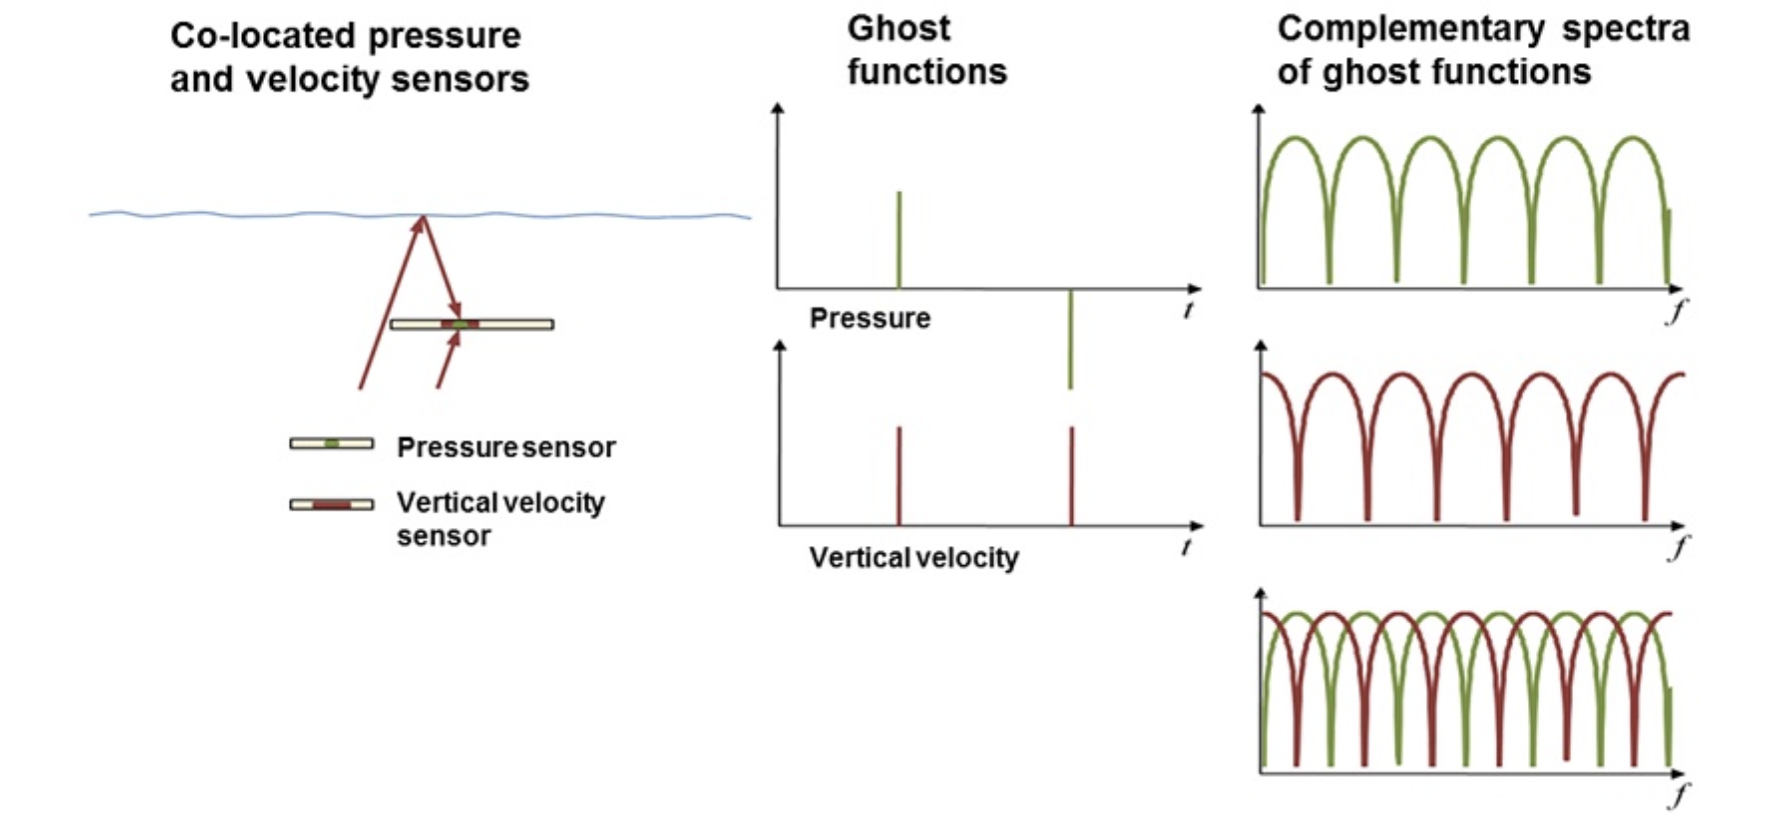
\includegraphics[width=1.0\textwidth]{Fig/ghost1.png}
\end{figure}
\end{frame}
%==============================================
\begin{frame}{U-D deghosting}
%==============================================
\begin{figure}
    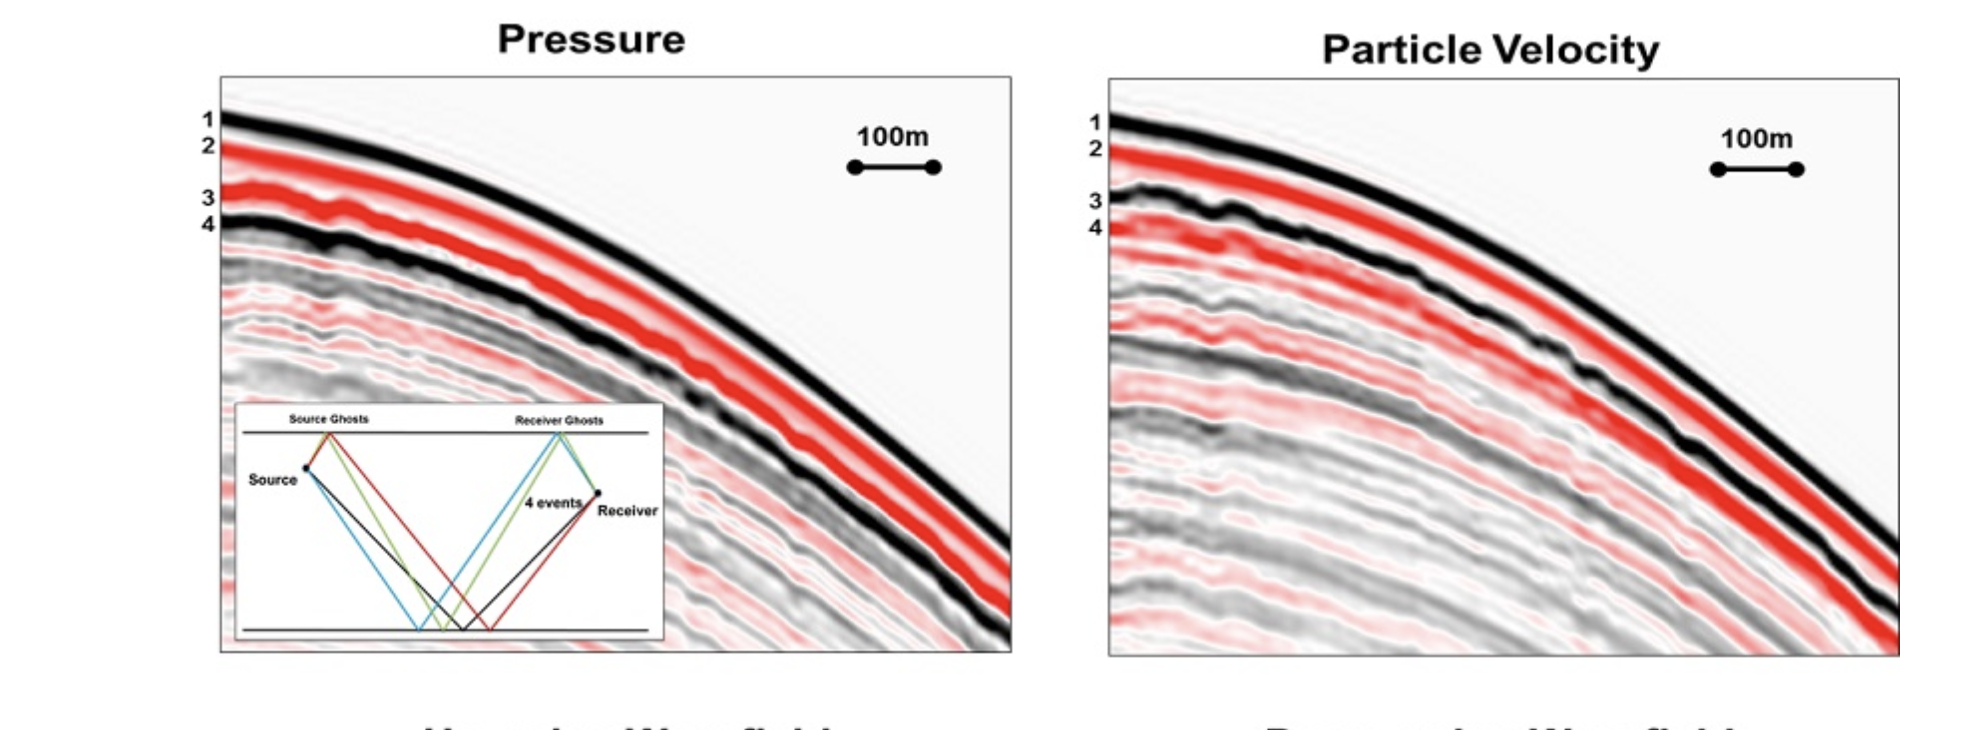
\includegraphics[width=1.0\textwidth]{Fig/ghost2.png}
\end{figure}
\end{frame}
%==============================================
\begin{frame}{U-D deghosting}
%==============================================
\begin{figure}
    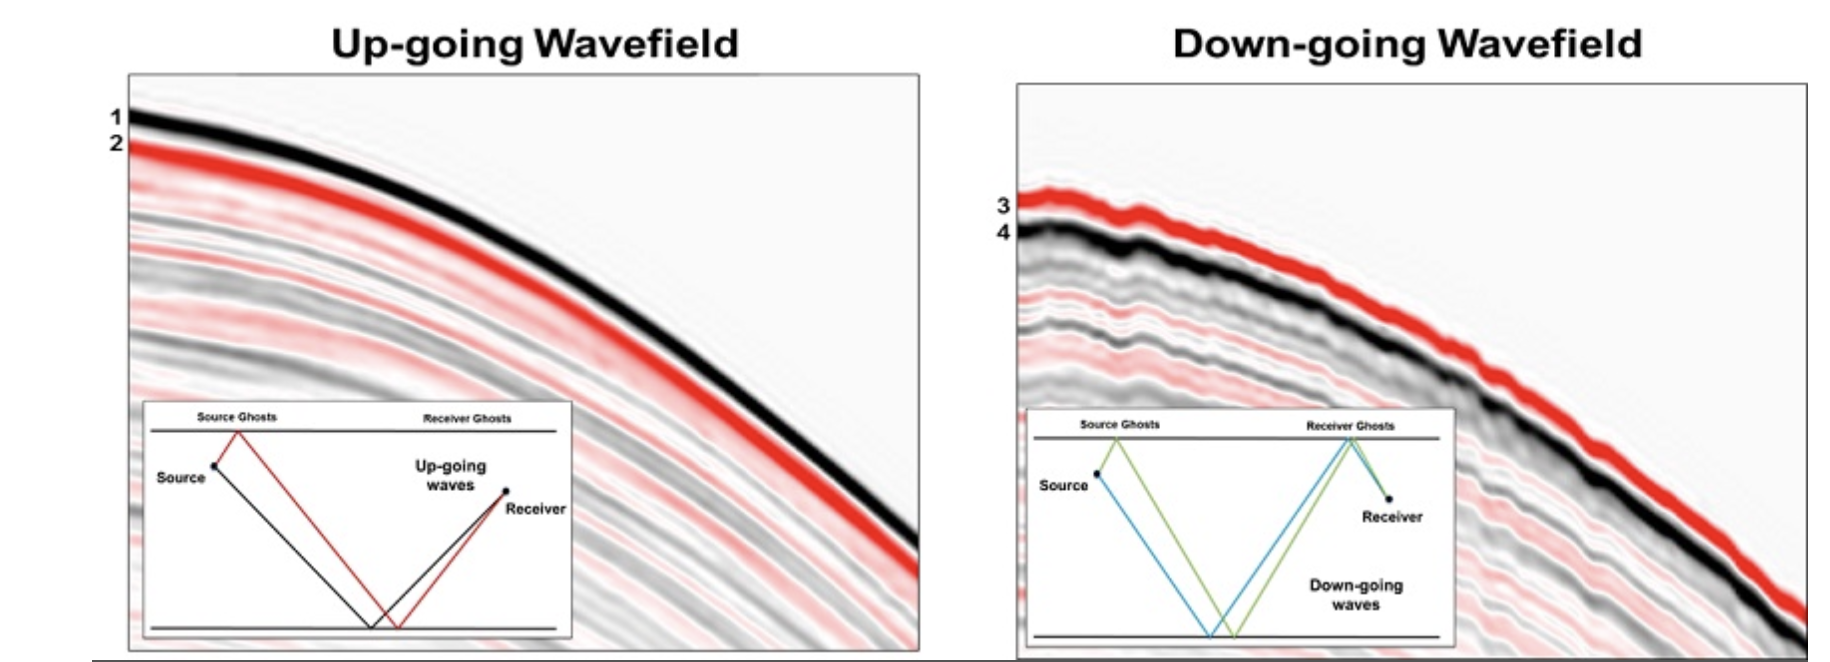
\includegraphics[width=1.0\textwidth]{Fig/ghost3.png}
\end{figure}
\end{frame}
\end{document}
%==============================================
\begin{frame}{U-D deghosting}
%==============================================
\begin{figure}
    \includegraphics[width=1.0\textwidth]{Fig/ghost4.png}
\end{figure}
\end{frame}
\end{document}
